\documentclass{beamer}
\usepackage{booktabs}
\usepackage{caption}
\usepackage[export]{adjustbox}
\graphicspath{ {./img/} }


\title{Travail Économétrique}
\subtitle{La part des locataires}
\author{Mosse Joseph, Rubira Pierre}
\institute{Univeristé de Montpellier \\Faculté d'économie}
\date{2022}

\usetheme{SimplePlus}
\setbeamertemplate{navigation symbols}{}
\usefonttheme[onlymath]{serif}
\begin{document}

\frame{\titlepage}

\begin{frame}
\frametitle{La part de locataires}
\begin{columns}
    
\begin{column}{0.5\textwidth}
\begin{table}[H]
    \begin{tabular}{cccc}
    \toprule
    Moyenne  & Écart-type   \\ 
    36,47 & 6,77    \\
    \midrule
    Minimum & Maximum   \\ 
    24,3    & 61,7     \\
    \bottomrule
    \end{tabular}
\end{table}
\end{column}
\begin{column}{0.5\textwidth}
    \centering
    \begin{figure}
        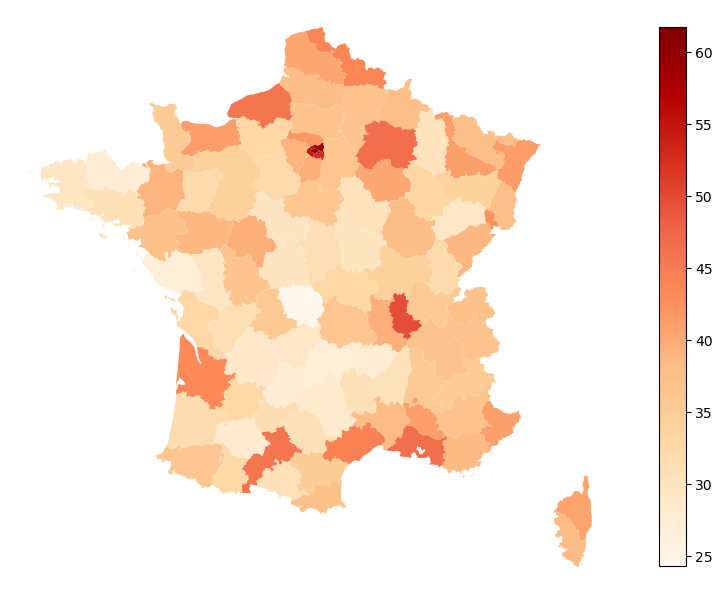
\includegraphics[width=\textwidth]{locataire.png}
        \caption{Part des locataires en 2019}
    \end{figure}
\end{column}
\end{columns}
\end{frame}

\begin{frame}
\frametitle{La part des diplômés}
\begin{columns}
\begin{column}{0.5\textwidth}
    \centering
    \begin{figure}
        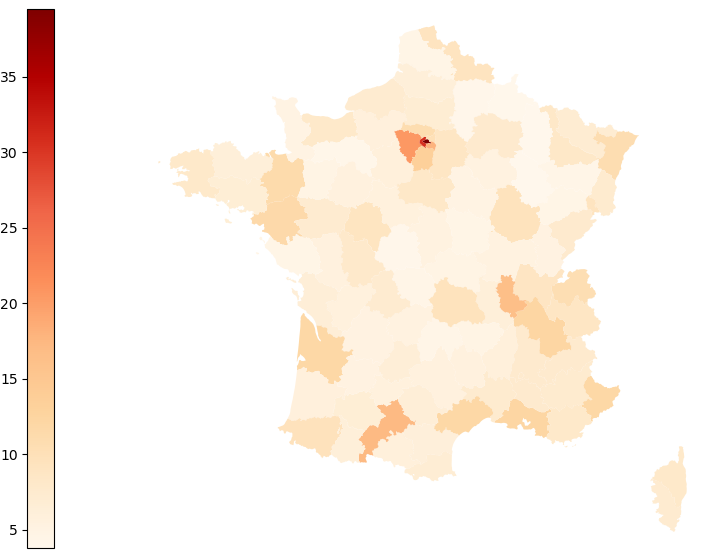
\includegraphics[width=\textwidth]{dipsup.png}
        \caption{Part des diplômés BAC+5 ou plus en 2019}
    \end{figure}
\end{column}

\begin{column}{0.5\textwidth}
\begin{table}[H]
    \caption*{Statistiques sur $dipsup$}
    \begin{tabular}{cccc}
    \toprule
    Moyenne  & Écart-type   \\ 
    8,14 & 5,10   \\
    \midrule
    Minimum & Maximum   \\ 
    3,8    & 39,5      \\
    \bottomrule
    \end{tabular}
\end{table}
\end{column}

\end{columns}
\end{frame}

\begin{frame}
    \frametitle{La part d'appartements}
    \begin{columns}
    
    \begin{column}{0.5\textwidth}
    \begin{table}[H]
        \caption*{Statistiques sur $appart$}
        \begin{tabular}{cccc}
        \toprule
        Moyenne  & Écart-type   \\ 
        35,86 & 17,26   \\
        \midrule
        Minimum & Maximum   \\ 
        12,9    & 96,9      \\
        \bottomrule
        \end{tabular}
    \end{table}
    \end{column}

    \begin{column}{0.5\textwidth}
        \centering
        \begin{figure}
            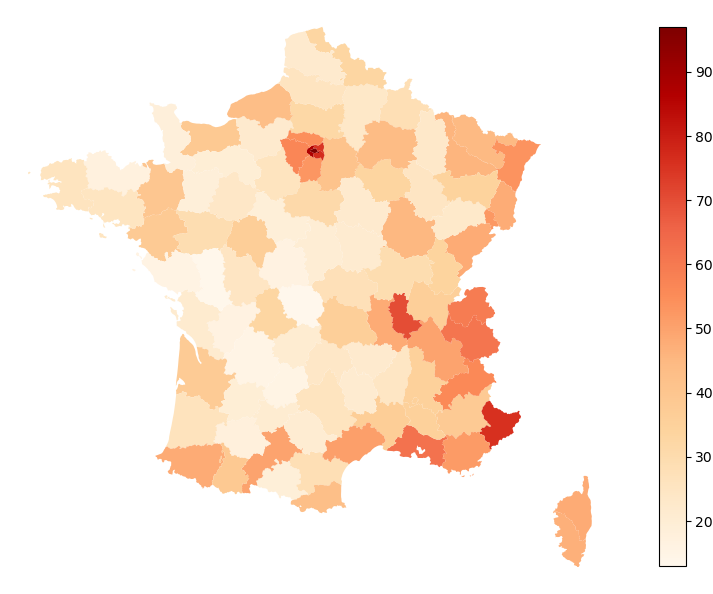
\includegraphics[width=\textwidth]{appart.png}
            \caption{Part des appartements en 2019}
        \end{figure}
    \end{column}
    
    \end{columns}
\end{frame}

\begin{frame}
\frametitle{Le taux de chômage}
\begin{columns}
\begin{column}{0.5\textwidth}
    \centering
    \begin{figure}
        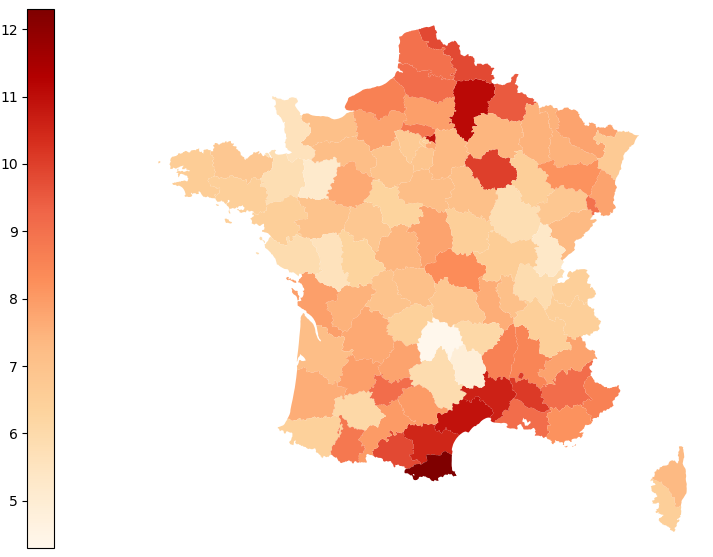
\includegraphics[width=\textwidth]{chomage.png}
        \caption{Taux de chômage en 2019}
    \end{figure}
\end{column}

\begin{column}{0.5\textwidth}
\begin{table}[H]
    \caption*{Statistiques sur $chomage$}
    \begin{tabular}{cccc}
    \toprule
    Moyenne  & Écart-type   \\ 
    7,55 &  1,47   \\
    \midrule
    Minimum & Maximum   \\ 
    4,3    & 12,3      \\
    \bottomrule
    \end{tabular}
\end{table}
\end{column}

\end{columns}
\end{frame}
    
\begin{frame}
    \frametitle{Le taux d'urbanisation}
    \begin{columns}
    
    \begin{column}{0.5\textwidth}
    \begin{table}[H]
        \caption*{Statistiques sur $urba$}
        \begin{tabular}{cccc}
        \toprule
        Moyenne  & Écart-type   \\ 
        68,07 & 17,62   \\
        \midrule
        Minimum & Maximum   \\ 
        21,4    & 100      \\
        \bottomrule
        \end{tabular}
    \end{table}
    \end{column}

    \begin{column}{0.5\textwidth}
        \centering
        \begin{figure}
            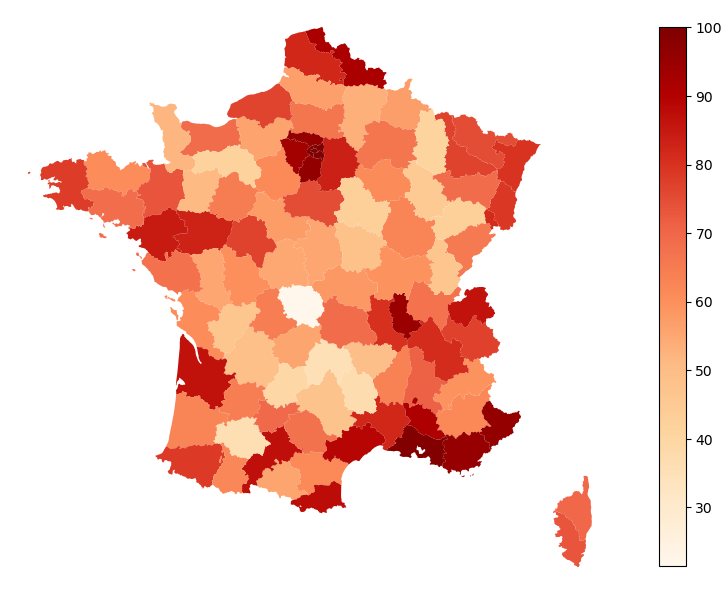
\includegraphics[width=\textwidth]{urba.png}
            \caption{Taux d'urbanisation en 2019}
        \end{figure}
    \end{column}
    
    \end{columns}
\end{frame}

\begin{frame}
    \frametitle{La part de personnes âgées}
    \begin{columns}
    \begin{column}{0.5\textwidth}
        \centering
        \begin{figure}
            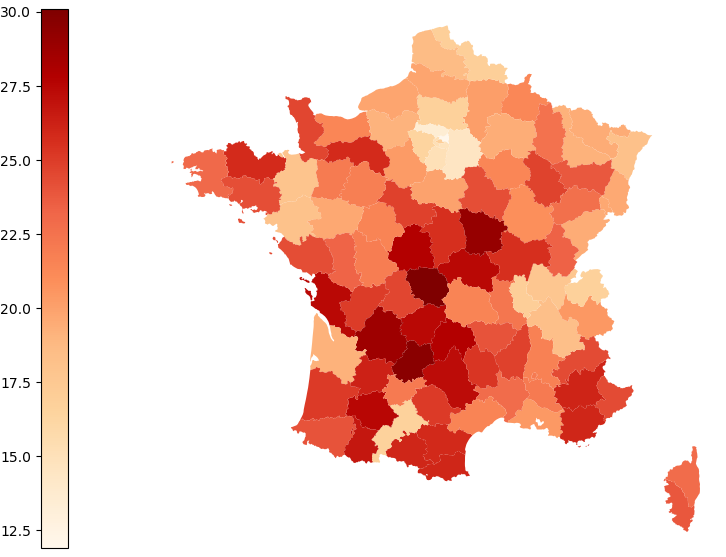
\includegraphics[width=\textwidth]{persagee.png}
            \caption{La part des personnes âgées de 65 ans ou plus en 2019}
        \end{figure}
    \end{column}
    
    \begin{column}{0.5\textwidth}
    \begin{table}[H]
        \caption*{Statistiques sur $persagee$}
        \begin{tabular}{cccc}
        \toprule
        Moyenne  & Écart-type   \\ 
        22,17 &  3,94   \\
        \midrule
        Minimum & Maximum   \\ 
        11,9    & 30,1      \\
        \bottomrule
        \end{tabular}
    \end{table}
    \end{column}
    
    \end{columns}
\end{frame}

\begin{frame}
    \frametitle{Le taux de pauvreté}
    \begin{columns}
    
    \begin{column}{0.5\textwidth}
    \begin{table}[H]
        \caption*{Statistiques sur $pauvrete$}
        \begin{tabular}{cccc}
        \toprule
        Moyenne  & Écart-type   \\ 
        14,37 & 2,99   \\
        \midrule
        Minimum & Maximum   \\ 
        9,1    & 27,9      \\
        \bottomrule
        \end{tabular}
    \end{table}
    \end{column}

    \begin{column}{0.5\textwidth}
        \centering
        \begin{figure}
            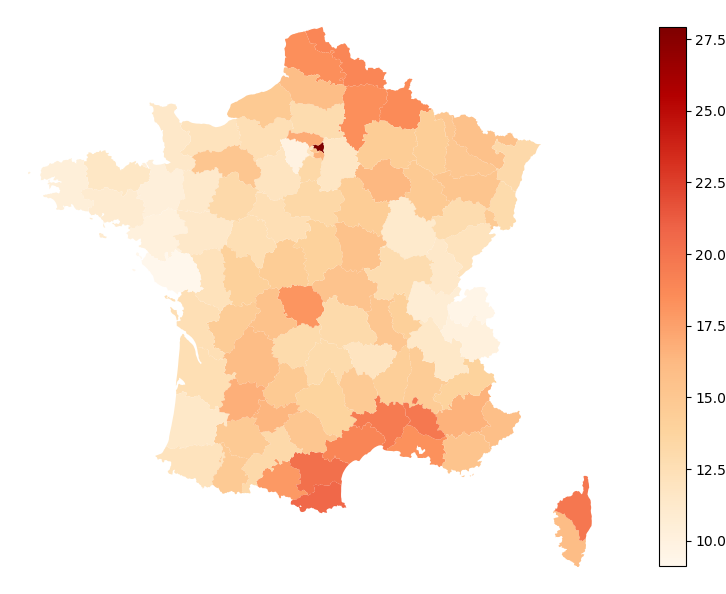
\includegraphics[width=\textwidth]{pauvrete.png}
            \caption{Taux de pauvreté en 2019}
        \end{figure}
    \end{column}
    
    \end{columns}
\end{frame}

\begin{frame}
    \frametitle{La part de jeunes}
    \begin{columns}
    \begin{column}{0.5\textwidth}
        \centering
        \begin{figure}
            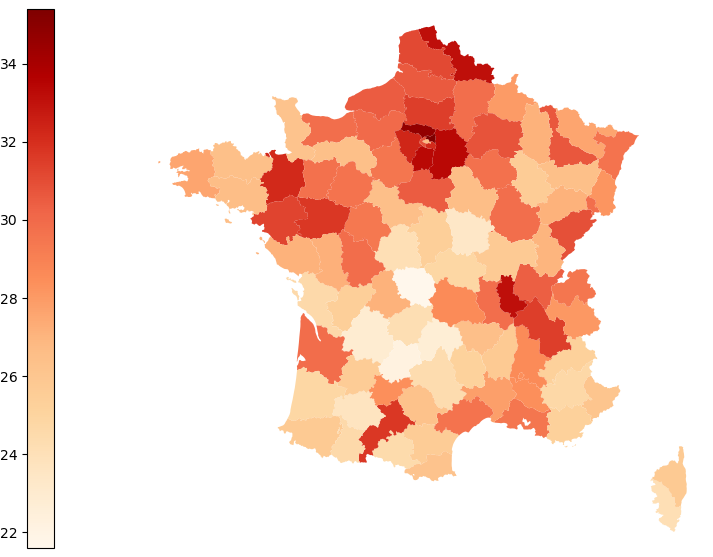
\includegraphics[width=\textwidth]{jeune.png}
            \caption{La part des personnes âgées de moins de 25 ans en 2019}
        \end{figure}
    \end{column}
    
    \begin{column}{0.5\textwidth}
    \begin{table}[H]
        \caption*{Statistiques sur $jeune$}
        \begin{tabular}{cccc}
        \toprule
        Moyenne  & Écart-type   \\ 
        27,99 &   2,98   \\
        \midrule
        Minimum & Maximum   \\ 
        21,6    & 35,4      \\
        \bottomrule
        \end{tabular}
    \end{table}
    \end{column}
    
    \end{columns}
\end{frame}

\begin{frame}
    \frametitle{Coefficients de corrélation des variables}
    \begin{figure}
        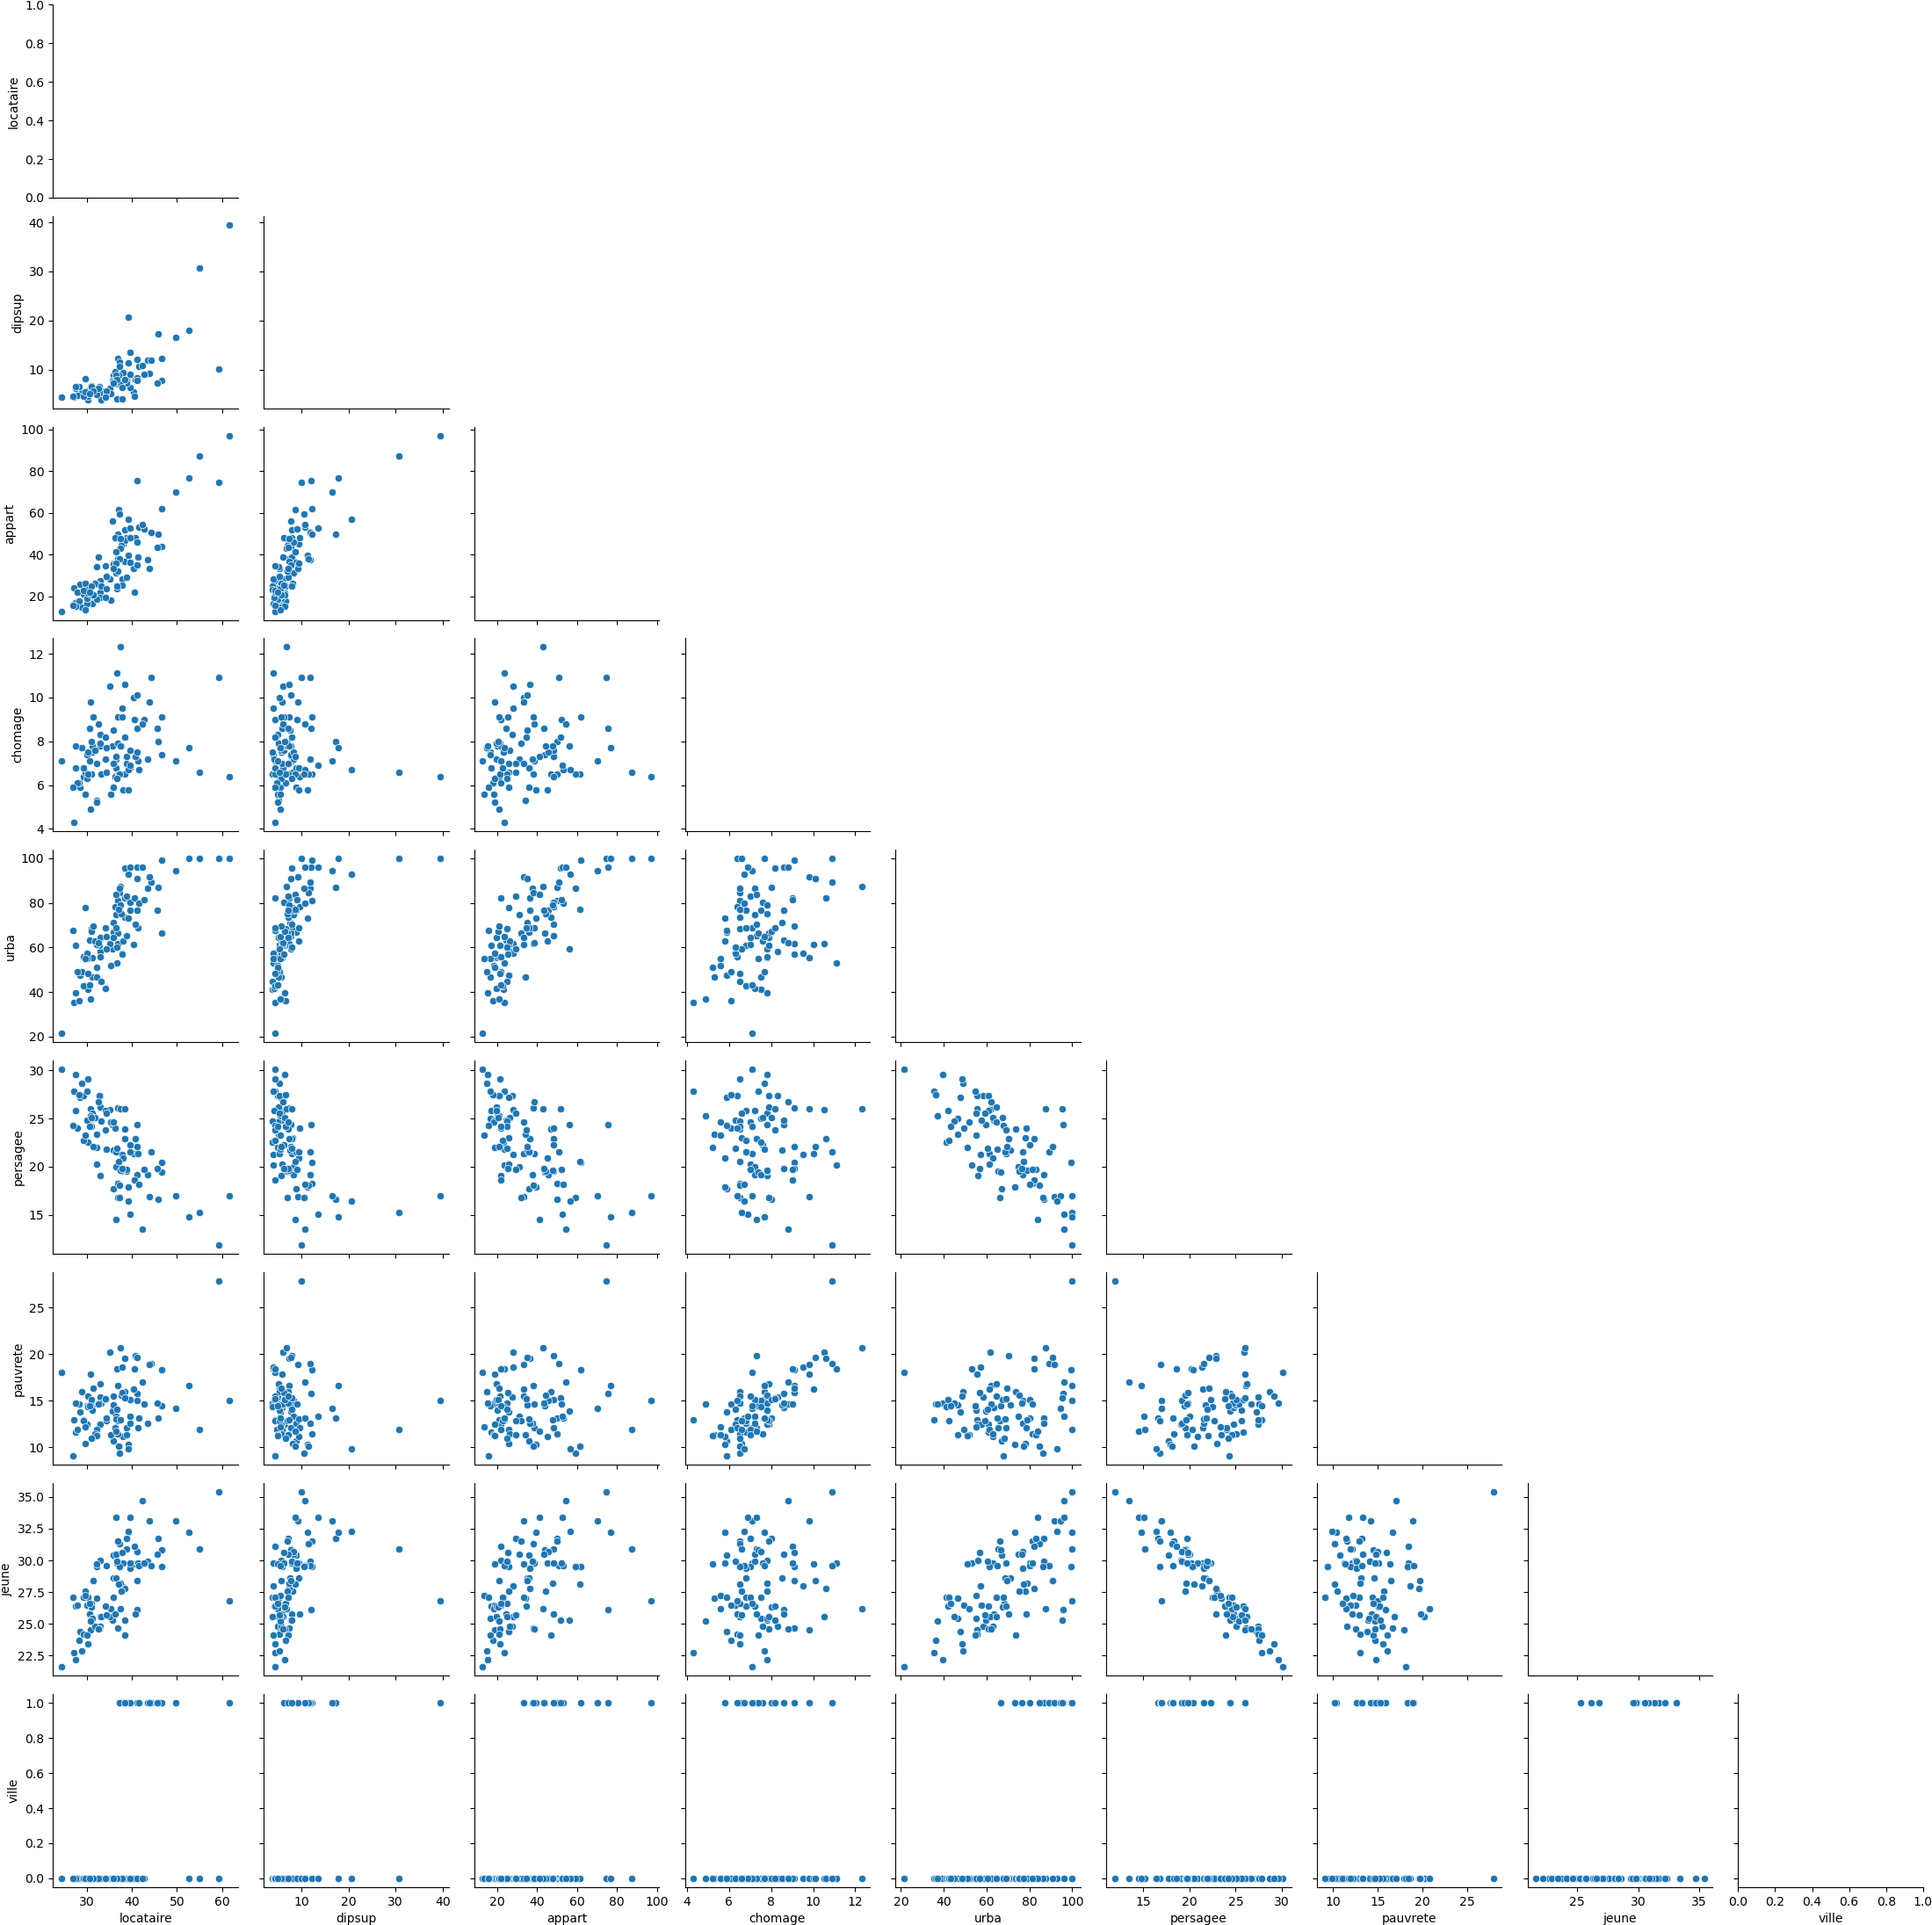
\includegraphics[max height=187px,max width=187px]{corr.png}
         \caption{Corrélation entre les différentes variables du modèle}
    \end{figure}
\end{frame}
\end{document}